\section{ISO/IEC 9126:2001}\label{ISO/IEC 9126Section}

L'ISO/IEC 9126:2001 individua un'insieme di normative e linee guida al fine di descrivere un modello di qualità del software. \`E scomposto in quattro parti, ciascuna delle quali si occupa di un diverso ambito. 
\begin{itemize}
	\item \textbf{Modello di Qualità}: insieme di caratteristiche di qualità che sono in grado di descrivere i principali fattori di qualità di un prodotto software, si possono classificare in: funzionalità, affidabilità, efficienza, usabilità, manutenibilità, portabilità;
	\item \textbf{Qualità Esterne}: insieme di metriche che misurano i comportamenti del software sulla base di test, dell'operatività e dal monitoraggio durante la sua esecuzione;
	\item \textbf{Qualità Interne}: insieme di metriche che si applicano alla qualità del software "non eseguibile", in sostanza al codice sorgente, durante la fase di sviluppo e pianificazione; l'obiettivo di queste metriche è scovare eventuali difetti, e prevedere la qualità finale attraverso misurazioni e strumenti che simulano il comportamento finale del prodotto;
	\item \textbf{Qualità in Uso}: rappresenta il punto di vista dell'utente; il livello corrente si raggiunge nel momento in cui tutte le qualità precedenti sono soddisfatte e quando l'utente è abilitato ad ottenere specificati obiettivi con:
	\begin{itemize}
		\item \textbf{Efficacia}: capacità del software di raggiungere obiettivi specificati con accuratezza e completezza;
		\item \textbf{Produttività}: capacità di mettere in grado l'utente di spendere una quantità di risorse appropriate per compiere una determinata azione in uno specificato ambito d'uso;
		\item \textbf{Sicurezza}: capacità del prodotto di raggiungere accettabili livelli di rischio per il software, apparecchiatura, persone;
		\item \textbf{Soddisfazione}: capacità del prodotto di soddisfare le attese degli utenti.
	\end{itemize}	
\end{itemize}
Le quattro parti sono legate strettamente da dipendenze importanti, il soddisfacimento di ognuna dipende dalla precedente. La seguente figura spiega al meglio il legame.

\begin{figure}[H]
\centering

	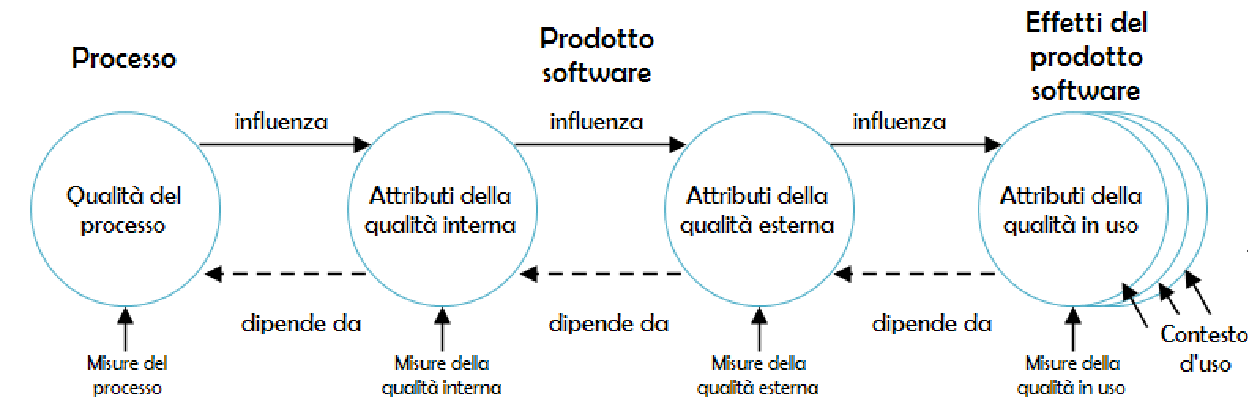
\includegraphics[width=0.9\linewidth]{./images/quality_cicle_iso9126.png} 
	\caption{ISO/IEC9126:2001. Immagine dal sito web \url{https://it.wikipedia.org/wiki/ISO/IEC_9126}}
	\label{ISO/IEC9126:2001}	

\end{figure}

 